% arara: pdflatex: { options: "--jobname great-name" }
\documentclass[12pt,a4paper]{report}
\usepackage[utf8]{inputenc}
\usepackage[margin=1.8cm]{geometry}
\usepackage{amsmath}
\usepackage[czech, slovak]{babel}
\usepackage{amsfonts}
\usepackage{amssymb}
\usepackage{graphicx}
\usepackage{lmodern}
\usepackage{enumitem}
\usepackage{listings}


\begin{document}



\begin{titlepage}

\fontfamily{qhv}\selectfont
\addtolength{\voffset}{-3cm}

\noindent\hspace{-60.0pt}\includegraphics[width=0.6\textwidth]{./img/VUT_symbol_barevne_CMYK_CZ}\\
\Large\textbf{VYSOKÉ UČENÍ TECHNICKÉ V BRNĚ}\\
\small\textbf{BRNO UNIVERSITY OF TECHNOLOGY}\\\vfill\hspace{-0.7cm}
\Large\textbf{FAKULTA INFORMAČNÍCH TECHNOLOGIÍ}\\
\small\textbf{FACULTY OF INFORMATION TECHNOLOGY}\\\vfill\hspace{-0.7cm}
\Large\textbf{IFJ - DOKUMENTACE PROJEKTU}\\
\small\textbf{IFJ - PROJECT DOCUMENTATION}\\\vfill\hspace{-0.7cm}
\Large\textbf{SEMESTRÁLNÍ PROJEKT}\\
\small\textbf{TERM PROJECT}\\\vfill\hspace{-0.7cm}
\Large\textbf{AUTORI PRÁCE \hfill \normalsize{Marek Tamaškovič, Martin Vaško,}}\\
\small\textbf{AUTHORS} \hfill \normalsize\textbf{Michal Vaško, Jiří Záleský, Jakub Zárybnický}
\vfill\hspace{-0.7cm}
\large\textbf{BRNO 2017}

\newpage
\fontfamily{\familydefault}\selectfont%
\end{titlepage}

\newgeometry{margin=2.5cm}

\begin{abstract}
Dokumentacia popisuje implementáciu interpretu jayzka IFJ16, ako podmnožinu jazyka java8, bez podpory objektového programovania.Projekt sa dá rozdeliť na štyri hlavné časti, z ktorých bude každej venovaná osobitná kapitola.
\begin{itemize}
\item Lexikálny analyzátor, ktorý zo zdrojového programu získava tokeny
\item Syntaktický analzátor, ktorý rozdeľujeme na dve podčasti- syntaktický analyzátor jazykových konštrukcií a na analyzátor výrazov.
\item Sémantický analyzátor, ktorý v zdrojovom programe zisťuje, či konštrukcie s ktorými sa pracuje v programe nachádzajú v globálnom resp. lokálnom priestore.
\item Interpret, ktorź ma za úlohu previesť interpretáciu programu.
\end{itemize}
\end{abstract}

\tableofcontents

\chapter{Štruktúra projektu}

\section{Lexikálna analýza}
Lexikálna analýza alebo teda Scanner funguje na princípe konečného automatu. Postupne načitáva  znaky zo vstupného súboru a posiela ich syntaktickému analýzatoru vo forme tokenov.Poslany token obsahuje informácie o type, obsahu a pozicii(riadok,stĺpec) na ktorej sa v interpretovanom subore nachádza.Všetky tieto informácie su potrebné pre uľahčenie práce parseru.V prípade ,že načítame niečo čo nezapadá do pravidiel programovacieho jazyka IFJ16 nastane lexikálna chyba. Náš scanner podporuje aj všetky dostupne a povolené rozšírenia ako napríklad unárne operatory či rozširenie BASE a dalšie. Diagram konečného automatu si možete prezrieť v priloženej prílohe.V diagrame došlo k  upravám, kvôli prehľadnosti stavov, preto stavy v diagrame úplne nezodpovedajú stavom v kóde.
\section{Syntaktická analýza}
\textbf{\textit{TODO}}
\section{Sémantická analýza}
Sémantická analýza kódu prebieha samostatne po syntaktickej analýze, z dôvodu jazyka IFJ16(Podmnožina java8), ktorý podporuje používanie staticky typovaných premenných aj v iných triedach.Dochádzalo by preto ku konfliktom(nevyplneným údajom v tabuľke symbolov) v prvom prechode syntaktickej analýzy. Rozšírenia ako CYCLES a BOOLOP museli rozšíriť sémantické kontroly o príkazy - break,continue, a rekurzívne spracovanie booleovských podmienok.
\section{Interpret}
Interpret má za úlohu vykonať to, čo sa nachádza v zdrojovom kóde interpretovaného programu. Náš interpret interpretuje abstraktný syntaktický strom, ktorý vytvorila syntaktická analýza. Ten lineárne prechádza a vyhodnocuje výrazy pokým nenastane volanie funkcie. V tom momente si vyhľadá v tabuľke symbolov abstraktný syntaktický strom danej funkcie, vytvorí lokálnu tabuľku symbolov, ktorú bude používať volaná funkcia, vloží do nej argumenty funkcie a začne vykonávať telo funkcie. Pri ukončovaní funkcie interpret vloží návratovú hodnotu z funkcie na zásobník a ukončí interpretáciu funkcie. Následne si interpret danú hodnotu vyberie zo zásobníka a použije ju v interpretácii pôvodného abstraktného syntaktického stromu. Vstavané funkcie sú riešené obdobne. Taktiež si pri interpretácii interpret kontroluje behové chyby ako napríklad delenie nulou alebo práca s neinicializovanými premennými. Ak taká situácia nastane interpret sa ukončuje s chybovou hláškou a príslušným návratovým kódom pre danú chybu.

\section{Garbage collector}
\par Pro lepší správu paměti jsme implementovali garbage collector. Je implementován jako statické pole struktury obsahující void ukazatel a ukazatel na další prvek stejného typu. Což umožňuje za sebou prvky řadit jako lineární spojový seznam. Po naalokování paměti je volána funkce, která vytvoří nový prvek. Na základě adresy je posléze pomocí hashovací funkce určeno nové umístění prvku. Je-li již na daném umístění nějaký prvek, je umístěn za poslední prvek v pořadí. Při mazání prvku je použita hashovací funkce a následným porovnáváním se najde daný prvek ve spojovém seznamu a po přepojení prvků je paměť, a následně i prvek, uvolněna.
\par Součástí jsou i modifikované funkce pro alokoci, realokaci a dealokaci paměti. Ve funkcích pro alokaci a realokaci je také kontrola toho, zda alokace proběhla úspěšně.

\section{Algoritmy}
% Nejak zvýraznit názvy funkcí?
\subsection{List-Merge sort}
\par Metoda řazení pole využívající princip slučování (mergování) seznamů.
V první fázi je vytvořeno pomocné pole indexů, které je následně využito pro najití začátků neklesajících poslupností. Konec posloupnosti je v pomocném poli vyznačen pomocí 0. Začátek každé posloupnosti je uložen do pomocné datové struktury typu seznam a přidán do fronty.
\par Ve fázi druhé, pak vždy vezmene první dva prvky fronty a seřadíme je. Z těchto dvou prvků vznikne jeden větší, který umístíme na konec fronty. Takto postupujeme dokud nezůstane ve frontě pouze jeden seznam, který je výsledkem řazení. Pro větší jednoduchost kódu, je před spojováním a řazením zaručeno pořadí tak, aby seznam obsahující nižší index byl vždy první z dvojice pro seřazení.

\subsection{KMP Vyhledání podřetězce}
\par Knuth-Morris-Prattův algoritmus se využívá pro urychlení hledání výskytu stejných podřetězců v hledaném řetězci. Algoritmus využívá pomocného pole obsahující informace o hledaném podřetězci. Toto pole musí být vytvořeno ještě předtím než je zahájeno hledání. Složitost algoritmu je $\mathcal{O}(n)$.
\par V první fázi je zavolána pomocná funkce Prefixcreator, která do pomocného pole uchovávajícího pozice od kterých se má pokračovat ve porovnávání, umístí hodnoty na základě nalezených podřetězců. Není-li podřetězec větší než 1 pak je pomocná tabulka vyplněna -1.
Ve fázi druhé již probíhá porovnávání hledaného řetězce s řetězcem vstupním. Výsledkem je pozice na, které začíná hledaný řetězec.


\subsection{Binárny vyhľadávací strom - BVS}
\par Pre vkladanie premenných,funkcii a tried sme v zadaní využili binárny vyhľadávací strom AVL. Základom stromu je vloženie a nájdenie uzlu.Vrámci vloženia navyše strom vyvažujeme čo uľahčuje následne vyhľadanie uzlu v strome.Pre vkladanie máme 3 typy uzlov- uzly pre vstavané funkcie, uzly pre jednoduchú sémantickú kontrolu a uzly s konkrétnymi hodnotami.Pre jazyk IFJ16 sme zaviedli aj vyhľadávanie v dvoch stromoch naraz(lokálny a globálny) spolu so zistením mena triedy, z dôvodu rovnakých názvov funkcií vrámci rôznych tried.
\par Vkladanie je založené na porovnávaní kľúčov. Ak je kľúč ktorý vkladáme menší(v abecede viac naľavo) vkladáme do ľavého uzlu podstromu, inak vkladáme do pravého uzlu podstromu. Pri zhode kľúčov nastáva sémanticka chyba z dôvodu možného pretypovania už existujucého kľúča(názvu funkcie, premennej alebo triedy)

\chapter{Vývoj}

\section{Rozdelenie práce}
\begin{itemize}
\item \textbf{Martin Vaško} - Algoritmy(BVS),sémantické kontroly,testovanie,správa, návrh a výpomoc vrámci interpretu.
\item \textbf{Marek Tamaškovič} - Interpretácia AST, dokumentácia, garbage-collector,testovanie.
\item \textbf{Michal Vaško} - Lexikálny analyzátor,dokumentácia,prezentácia.
\item \textbf{Jiří Záleský} - Algoritmy(List-Merge sort,KMP), sémantické kontroly, vstavané funkcie, testovanie.
\item \textbf{Jakub Zárybnický} - Parser, precedenčná a syntaktická analýza, návrh, rozdelenie práce a štýl kódu.
\end{itemize}

\section{Komunikačné kanály}
\par Online komunikácia prebiehala v 3 typoch - pre rozdelenie práce sme používali \textbf{Trello}\footnote{https://trello.com/} kde sme si rozdeľovali nové úlohy, rozšírenia a detaily. Pre menej formálnu komunikáciu a výpomoc navzájom sme sa stretávali na komunikačnom kanály \textbf{Slack}\footnote{https://slack.com/} - kde sme si spisovali blížiace sa termíny a do osobitnej zložky \#announcements sa nám zasielal výpis z prekladu \textbf{Travis-CI}\footnote{https://travis-ci.org/}.
\par Ako verzovací systém sme si zvolili \textbf{Git}\footnote{https://git-scm.com/}.
\par Ako tím sme mali naplánované stretnutia pravidelne každé 2 až 3 týždne, kde sme preberali náš aktuálny stav a prognózu do ďalších dní, riešili rozhrania jednotlivých modulov a implementáciu rozšírení.

\chapter{Záver}
Tento projekt, implementácia interpretu IFJ16, bol veľkou výzvou hlavne po kooperatívnej stránke. Najväčsí problém pri kooperácii bolo zdielanie zdrojových kódov,cez verziovací systém, ktorý sme sa ku koncu projektu naučili lepšie používať. Náš interpret bol testovaný viacerými testami z vlastnej dielne a taktiež na viacerých operačných systémoch AntergOS, Fedora 22, Ubuntu 16.04.

\section{Metriky}

\begin{itemize}
\item Počet súborov: \textbf{24}
\item celkový počet riadkov zdrojového kódu: \textbf{8100}
\item Počet Git commitov: \textbf{380}
\end{itemize}


\chapter{Príloha}
\section{Diagram lexeru}
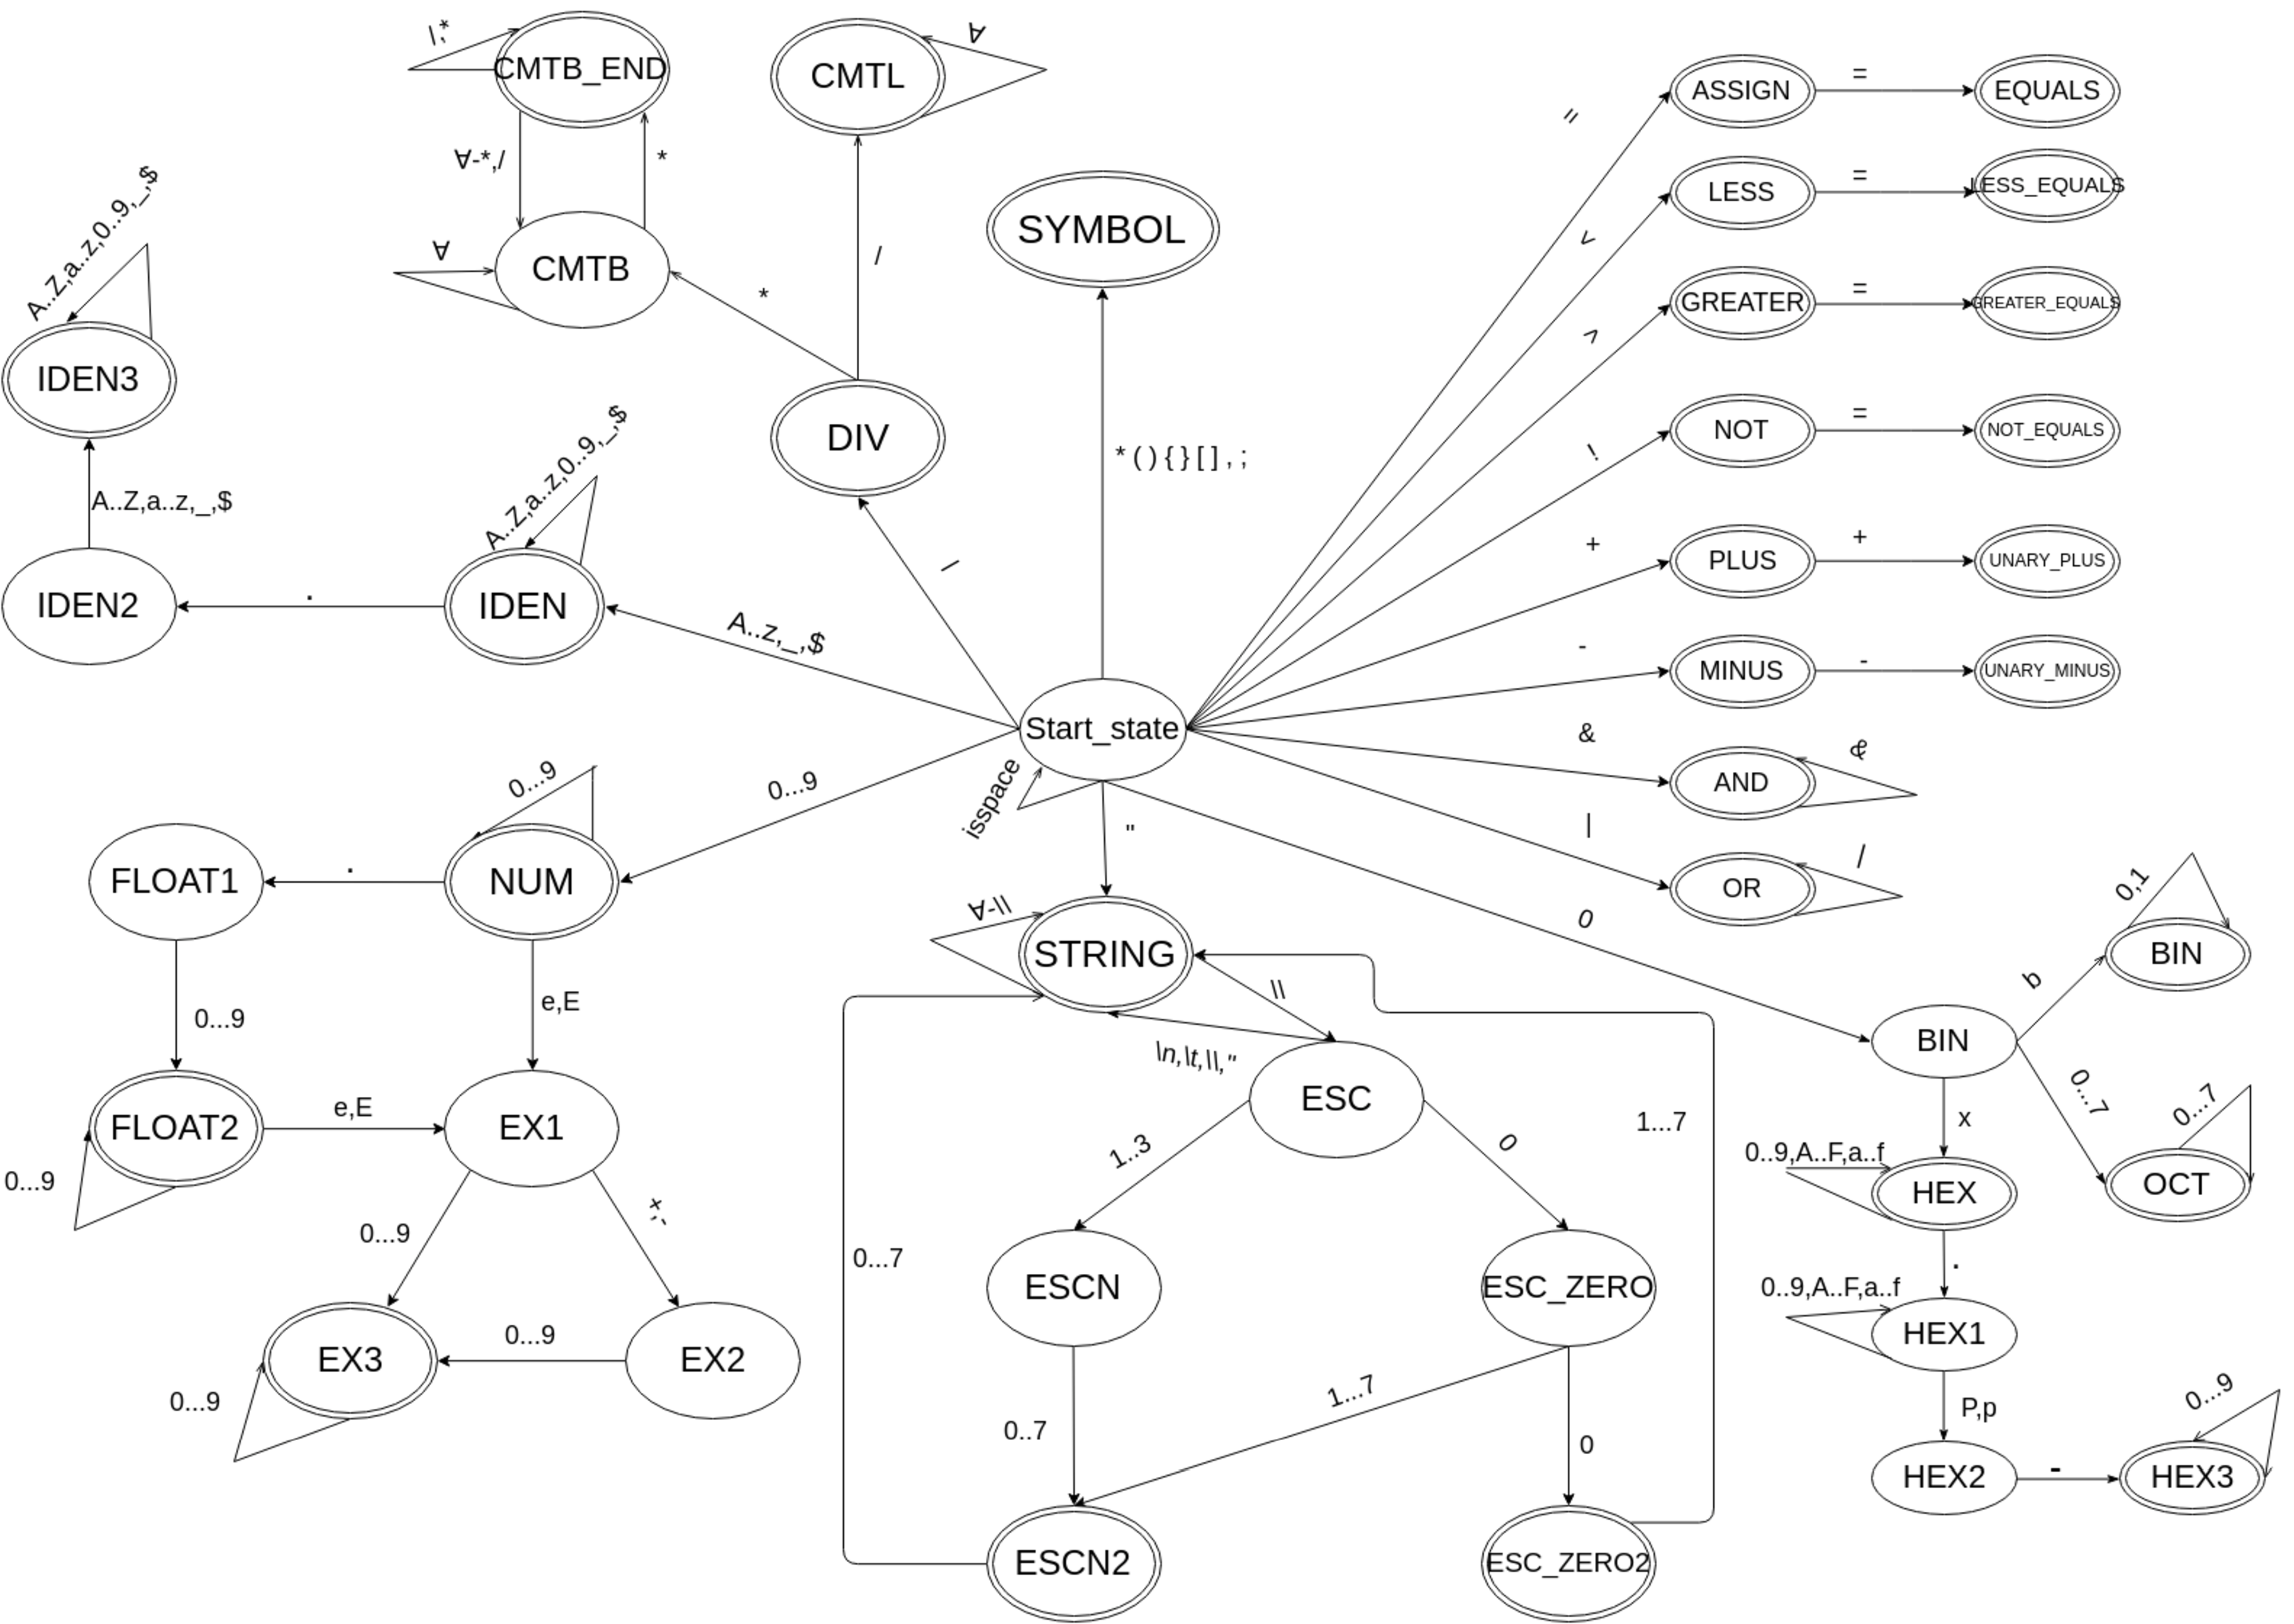
\includegraphics[width=1\textwidth]{./img/lex1.pdf}
\newpage
\section{LL gramatika}

\begin{lstlisting}
ifj16 = \$ | class ifj16
class = "class" "{" classBody
classBody = "}" | "static" type simpleId classBody'
classBody' = ";"
           | "=" expression ";"
           | "(" declarationList "{" functionBody
functionBody = "}"
             | type simpleId(q) functionBody'
             | command
functionBody' = ";" | "=" expression ";"
command = "if" "(" expression ")" command
        | "while" "(" expression ")" command
        | "do" command "while" "(" expression ")" ";"
        | "for" "(" type simpleId for'
        | "return" return'
        | "{" commandList
        | "break" ";"
        | "continue" ";"
        | anyId command'
for' = ";" for'' | "=" expression ";" for''
for'' = expression ";" anyId "=" expression ")" command
return' = ";" | expression ";"
commandList = "}" | command commandList
command' = "(" argumentList ";" | "=" expression ";"
declarationList  = ")" | type simpleId declarationList'
declarationList' = ")" | "," type simpleId declarationList'
argumentList  = ")" | expression argumentList'
argumentList' = ")" | "," expression argumentList'
type = "int" | "double" | "boolean" | "String" | "void"
anyId = simpleId | compoundId

expression = [see operator-precedence grammar]
\end{lstlisting}

\newpage

\section{Precedenční tabulka}

\scalebox{0.8}{
\begin{tabular}[pos]{r|l|l|l|l|l|l|l|l|l|l|l|l|l|l|l|l|l|l|l|l|l|l|l}
    &(&)&++&--&u-& !& *& /& +& -& <& >&<=&>=&==&!=&\&\&&$\|$&id&li&tf&,& \$ \\
    (& L& E& L& L& L& L& L& L& L& L& L& L& L& L& L& L& L& L& L& L& L& E& O \\
    )& O& G& O& O& O& O& G& G& G& G& G& G& G& G& G& G& G& G& O& O& O& G& G \\
    ++& O& G& G& G& O& O& G& G& G& G& G& G& G& G& G& G& G& G& L& O& O& G& G \\
    --& O& G& G& G& O& O& G& G& G& G& G& G& G& G& G& G& G& G& L& O& O& G& G \\
    u-& L& G& O& O& G& G& G& G& G& G& G& G& G& G& G& G& G& G& L& G& L& O& G \\
    !& L& G& O& O& G& G& G& G& G& G& G& G& G& G& G& G& G& G& L& G& L& O& G \\
    *& L& G& L& L& L& L& G& G& G& G& G& G& G& G& G& G& G& G& L& L& L& G& G \\
    /& L& G& L& L& L& L& G& G& G& G& G& G& G& G& G& G& G& G& L& L& L& G& G \\
    +& L& G& L& L& L& L& L& L& G& G& G& G& G& G& G& G& G& G& L& L& L& G& G \\
    -& L& G& L& L& L& L& L& L& G& G& G& G& G& G& G& G& G& G& L& L& L& G& G \\
    <& L& G& L& L& L& L& L& L& L& L& G& G& G& G& G& G& G& G& L& L& L& G& G \\
    >& L& G& L& L& L& L& L& L& L& L& G& G& G& G& G& G& G& G& L& L& L& G& G \\
    <=& L& G& L& L& L& L& L& L& L& L& G& G& G& G& G& G& G& G& L& L& L& G& G \\
    >=& L& G& L& L& L& L& L& L& L& L& G& G& G& G& G& G& G& G& L& L& L& G& G \\
    ==& L& G& L& L& L& L& L& L& L& L& L& L& L& L& G& G& G& G& L& L& L& G& G \\
    !=& L& G& L& L& L& L& L& L& L& L& L& L& L& L& G& G& G& G& L& L& L& G& G \\
    \&\&& L& G& L& L& L& L& L& L& L& L& L& L& L& L& L& L& G& G& L& L& L& G& G \\
    $\|$& L& G& L& L& L& L& L& L& L& L& L& L& L& L& L& L& L& G& L& L& L& G& G \\
    id& E& G& G& G& O& O& G& G& G& G& G& G& G& G& G& G& G& G& O& O& O& G& G \\
    literal& O& G& O& O& O& O& G& G& G& G& G& G& G& G& G& G& G& G& O& O& O& G& G \\
    true/false& O& G& O& O& O& O& G& G& G& G& G& G& G& G& G& G& G& G& O& O& O& G& G \\
    ,& L& E& L& L& L& L& L& L& L& L& L& L& L& L& L& L& L& L& L& L& L& E& O \\
    \$& L& O& L& L& L& L& L& L& L& L& L& L& L& L& L& L& L& L& L& L& L& O& O
\end{tabular}
}
\end{document}
